\documentclass[12pt,a4paper,twoside]{report}

%%%%%%%%%%%%%%%%%%%%%%%%%%%%%%%%%%%%%%%%%%%%%%%%%%%%%%%%%%%%%%%%%%%%%%%%
%%%%%%%%%%%% Packages %%%%%%%%%%%%%%%%%%%%%%%%%%%%%%%%%%%%%%%%%%%%%%%%%%
%%%%%%%%%%%%%%%%%%%%%%%%%%%%%%%%%%%%%%%%%%%%%%%%%%%%%%%%%%%%%%%%%%%%%%%%

%%%%%%
% In general useful packages
%%%%%%
\usepackage[latin1]{inputenc} % allow Umlauts
\usepackage[T1]{fontenc} % Umlauts as character in font
\usepackage{fancyhdr}   % Header/Footer
\usepackage[pdftex]{graphicx}

%%%%%%
% The following packages are optional, uncomment them if useful and required
%%%%%%
\usepackage{fancyvrb}   % extended verbatim environment
% \usepackage{latexsym}   % additional symbols
% \usepackage{times}      % bessere Schrift in PS-Dateien
% \usepackage{longtable}  % long tables (with page breaks)
% \usepackage{breakcites}  % linebreaks in cites

\usepackage[us]{datetime} % date in \today as "Month DD, YYYY", e.g., "February 29, 2012"

%%%%%%
% Hyperlinks in PDF output (blue borders, text color unchanged)
%%%%%%
\usepackage[plainpages=false, pdfpagelabels, bookmarks,  colorlinks=false,
               linkbordercolor={0 0 1}, filebordercolor={0 0 1}, citebordercolor={0 0 1},
               menubordercolor={0 0 1}, pagebordercolor={0 0 1}, urlbordercolor={0 0 1}]{hyperref}

%%%%%%
% Another set of useful packages
%%%%%%
% \usepackage[square]{natbib}  % more powerful and customizable references
% \usepackage[center]{caption} % centered, multi-line captions of figures and tables
% \usepackage{floatflt}        % floats (e.g., figures & tables) which can have floating text around them
% \usepackage[thmmarks]{ntheorem}    % extended theorem environment
\usepackage{pdfcomment}  % comments in text as PDF notes

%%%%%%%%%%%%%%%%%%%%%%%%%%%%%%%%%%%%%%%%%%%%%%%%%%%%%%%%%%%%%%%%%%%%%%%%
%%%%%%%%%%%% Layout %%%%%%%%%%%%%%%%%%%%%%%%%%%%%%%%%%%%%%%%%%%%%%%%%%
%%%%%%%%%%%%%%%%%%%%%%%%%%%%%%%%%%%%%%%%%%%%%%%%%%%%%%%%%%%%%%%%%%%%%%%%
% German style (no paragraph indent, but gap between paragraphs)
% \setlength{\parindent}{0mm}
% \setlength{\parskip}{4pt plus3pt minus2pt}

% Page width and margins (usually no need to change, just use a4wide package)
% \setlength{\textwidth}{15cm}
% \addtolength{\oddsidemargin}{1mm}
% \addtolength{\evensidemargin}{-13.5mm}
\usepackage{a4wide} % better than individual setup

% For fancyhdr, otherwise it might result in "overfull vbox"
\addtolength{\headheight}{3.5pt}

% URL Prefix for Bibliography (i.e., no prefix, typewriter as font for URLs)
\newcommand{\urlprefix}{}
\def\UrlFont{\small\tt}
%\urlstyle{rm} % oder sf, falls obiges nicht funktioniert


%%%%%%%%%%%%%%%%%%%%%%%%%%%%%%%%%%%%%%%%%%%%%%%%%%%%%%%%%%%%%%%%%%%%%%%%
%%%%%%%%%%%% Some useful macros %%%%%%%%%%%%%%%%%%%%%%%%%%%%%%%%%%%%%%%%
%%%%%%%%%%%%%%%%%%%%%%%%%%%%%%%%%%%%%%%%%%%%%%%%%%%%%%%%%%%%%%%%%%%%%%%%

% myfigure: filename width caption
\newcommand{\myfigure}[3]{%
  \begin{figure}
    \centerline{\includegraphics[width=#2]{figures/#1.pdf}}
  \caption{#3}
  \label{fig:#1}
  \end{figure}
}

% Floating figures = figures with floating text around: filename width caption
\newcommand{\myfloatfigure}[3]{%
  \begin{floatingfigure}{#2}
    \includegraphics[width=#2]{figures/#1.pdf}
  \caption{#3}
  \label{fig:#1}
  \end{floatingfigure}
}

% two figures side by side: file1 width1 caption1 file2 width2 caption2
\newcommand{\mydoublefigure}[6]{%
  \begin{figure}
  \begin{minipage}[t]{#2}
    \centerline{\includegraphics[width=\textwidth]{figures/#1.pdf}}
  \centering
  \caption{#3}
  \label{fig:#1}
  \end{minipage}
  \hfill
  \begin{minipage}[t]{#5}
    \centerline{\includegraphics[width=\textwidth]{figures/#4.pdf}}
  \centering
  \caption{#6}
  \label{fig:#4}
  \end{minipage}
  \end{figure}
}


% Better verbatim environments (requires fancyvrb package)
\DefineVerbatimEnvironment{myverb}{Verbatim}{fontsize=\small,baselinestretch=0.84}
\DefineVerbatimEnvironment{myverbbox}{Verbatim}{frame=single,fontsize=\small,baselinestretch=0.84}


% For figures and tables
\renewcommand{\topfraction}{0.9} % a page has at most 90% of floats and at least 10% of text (if page contains floats AND text)
\renewcommand{\bottomfraction}{0.9}
\renewcommand{\floatpagefraction}{0.7} % a page with floats only is at least 70% full

% Hyphenation (include a special file with hyphenation hints if there are problems)
% \include{myhyphen}



\begin{document}

% Title page
\begingroup
  \pagenumbering{roman}
  \thispagestyle{empty}
%\setcounter{page}{1}

%\begin{figure}
%\begin{minipage}{.4\textwidth}
\parbox{0.5cm}{\ }
   \parbox{5.1cm}{
   
\includegraphics[width=4.5cm]{rwth.jpg}}
  \parbox{2cm}{
    
\includegraphics[width=1.2cm]{i5-300.jpg}}
    \parbox{1.2cm}{\ }
  \parbox{7cm}{
    
\includegraphics[width=6cm]{iais.jpg}}  
  % \end{minipage}
%\end{figure}

\vspace*{3cm}
\centerline{{\Large\bf Computing Distributed Representations }}

\vspace*{4mm}

\centerline{{\Large\bf for Polysemous Words}}

\vspace{2cm}

\centerline{Master Thesis}
% include the title of your programme
\centerline{Software Systems Engineering}

\vspace{2cm}

\centerline{{\large Haiqing Wang}}
\centerline{Matriculation number 340863}

\vspace{10mm}

% Date!
\centerline{\today}

\vspace{10mm}

\begin{center}
\begin{minipage}[t]{8cm}
Supervisors: \\
\hspace*{2cm} Prof. Dr. Gerhard Lakemeyer \\
\hspace*{2cm} Prof. Dr. Christian Bauckhage\\[1cm]
Advisors: \\
\hspace*{2cm} Dr. Gerhard Paaß\\
\hspace*{2cm} Dr. Jörg Kindermann\\
\end{minipage}
\end{center}



\endgroup

%%%%%%%%%%%%%%%%%%%
% Header & footers
%%%%%%%%%%%%%%%%%%%

\pagestyle{fancy}

% Headers with page numbers and section/chapter titles
\renewcommand{\sectionmark}[1]{\markright{\thesection\ #1}}
\renewcommand{\chaptermark}[1]{\markboth{\thechapter\ #1}{}}
\lhead[\rm\thepage]{\sl\rightmark}
\chead{}
\rhead[\sl\leftmark]{\rm\thepage}

% Footers empty
\lfoot{}
\cfoot{}
\rfoot{}


\tableofcontents

% Include also list of figures and tables if useful
%\listoffigures
%\listoftables


%%%%%%%%%%%%%%%%%%%%
%%% Contents %%%%%%%
%%%%%%%%%%%%%%%%%%%%
% Put each chapter in a separate file

\chapter{Introduction}
\label{cha:intro}

% Important: you have to switch to arabic numbering here!
\pagenumbering{arabic}

\begin{itemize}
\item Background / Context of the thesis
\item If applicable: describe the project the thesis is related to (e.g., CoCar)
\item Problem / Motivation
\item Goals of the thesis
\item For final thesis document: outline of the document
\end{itemize}

This is an example for a citation \cite{DBLP:journals/jods/KenscheQCJ07}.

\section{Figures}

Use vector graphics wherever possible and avoid bitmap images. Do not
use JPG at all (they are often blurred because of the compression). If
you have to include a bitmap graphics, use the PNG format. If you have
to use a JPG (as in the case for the logos on the title page), make sure
that these are images with high resolution and high quality.
\pdfcomment{pdfcomment is a useful package to put annotations like this one into the text.}

The preferred way to create a PDF image to be used in LaTeX is the following:
\begin{enumerate}
\item Do the image with your favorite graphics program (Powerpoint works well for many cases).
\item Print/Save the image as a PDF file (Acrobat Professional might be required, but
there also Open Source solutions, e.g. FreePDF)
\item Crop the image file and remove white margins.
\item Include it in LaTeX as in this example.
\end{enumerate}

How to refer to images:
Figure \ref{fig:labelOfFigure1} shows something from \cite{AfratiPODS2002}
whereas figure \ref{fig:labelOfNextFigure} is about \cite{LenzeriniPODS2002}.

If your image is not your own and taken from another source, cite the source
also in the caption.

% priority where to place the figure: here, top, bottom, page
\begin{figure}[htbp]
  % center the image.
  \centering

  % include a png file. Adapt size to 0.5 * textwidth and retain aspect ratio (!)
  \resizebox{\textwidth}{!}{
\includegraphics{Figure1.png}}

  \caption{The text under the figure \cite{AfratiPODS2002}}
  \label{fig:labelOfFigure1}
\end{figure}


\begin{figure}[htbp]
  \centering
  % Include a pdf file but make it a little smaller than the textwidth
  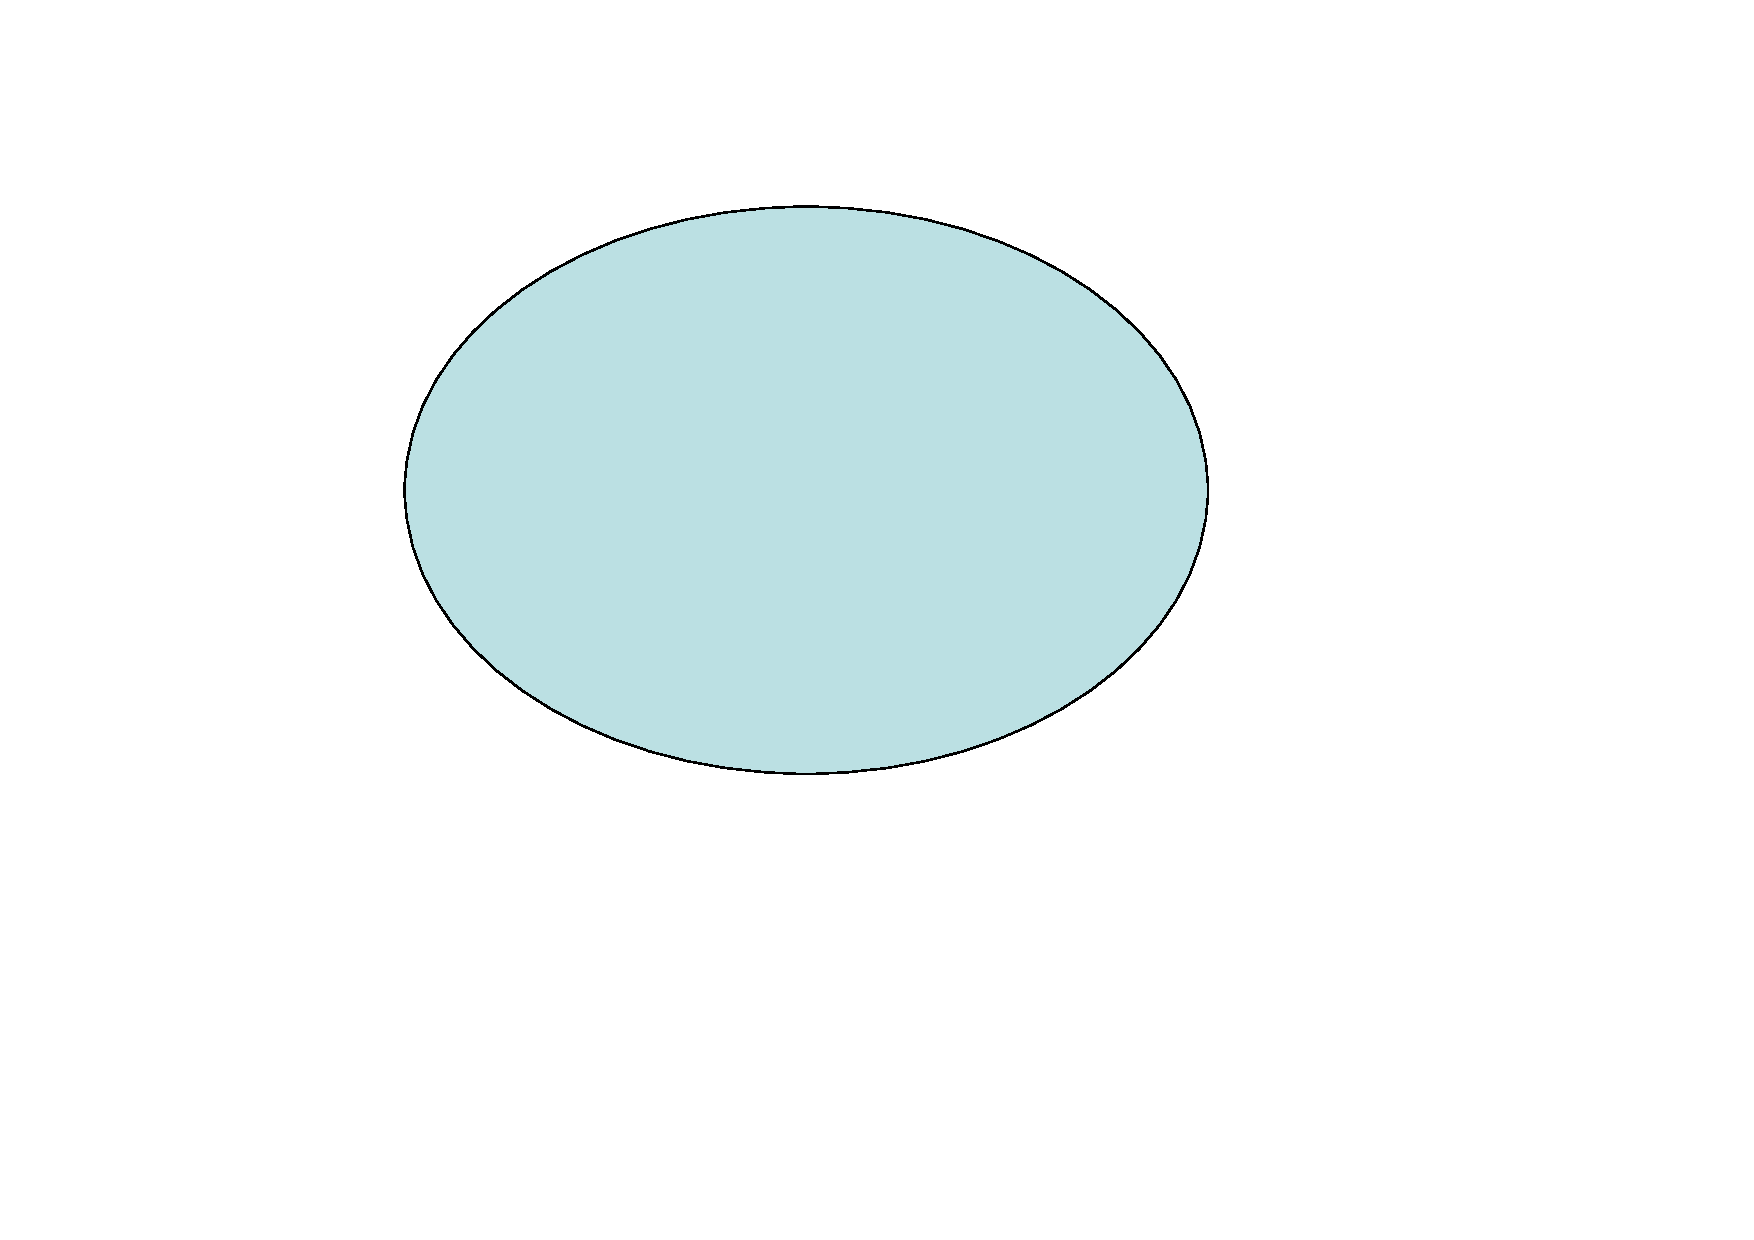
\includegraphics[width=0.5\textwidth]{Figure2.pdf}
  % Use EPS if you cannot create PDF files
  % (See http://www.wmf2eps.de.vu/ for creating eps files from powerpoint figures)
  \caption{Another text under this figure \cite{LenzeriniPODS2002}}
  \label{fig:labelOfNextFigure}
\end{figure}




\chapter{Related Work}
\label{cha:relwork}
This chapter introduces the related approaches for the inventor identification. These approaches can be classified into two categories. The first category is to make use of the inventor publications. In order to do that, the linkages between the inventors and the authors should be identified correctly. The second category is to leverage the information of the patent. This kind of approaches usually calculates the similarities between inventors to do the identification.


%Michele Pezzoni divides the inventor disambiguation into three steps: cleaning \& parsing, matching and filtering\cite{RePEc:grt:wpegrt:2012-29}. The cleaning \& parsing step removes the special characters from the inventor names such as punctuation, double blanks and etc. The remaining characters which are converted into ASCII codes. Then the string of the inventor name is parsed into several tokens such as surname, given name and etc. The similar process is also applied on the inventor address and the address is parsed into street, city and etc.The matching step is to match the inventors if they have a similar representation of the name. The filtering step is to decide which matching would be retained. A similarity score which is a sum of  seventeen weighted criterion is computed for each matching. The seventeen criterion could be divided into six categories: social network, geographical, applicant, technology, citation and others.  Compare this score to a threshold. If the score is larger than the threshold, the matching is retained otherwise it would be discarded.  This effectiveness of this approach is based on the quality of the data about the inventor while the clustering algorithm for my thesis is based on the contents of the patents and leverage the information of the publications which should be more robust.

\section{Identifying Author-inventors from Spain}
Maraut introduced an approach to match the inventor of the patent and the author of the publication from Spain \cite{iaifs}. The approach is divided into four steps. The first step is to struct the representations of the patents and the publications for names and addresses. The second step is to match the inventor and the author by using the names and the addresses. The address for the author is the institution address which the author is affiliated to while the addresses for the inventor are the addresses of the applicants and the inventors. The third step is to calculate a global similarity score which can be used to run a clustering to group the inventors and the authors. The inventors and the authors in the same cluster are considered as the same person. The fourth step is to control the data quality and improve the accuracy of the disambiguation manually by using recursive methods. For this approach, the weights used for the global similarity score and the threshold are calibrated manually. My approach leverages the texts of the patents and the publications to match them and identifies the weights and threshold by using the logistic regression.
%Maraut introduces an approach to match the inventor of the patent and the author of the publication from Spain\cite{iaifs}. The approach is divided into four steps. First step is to struct the name and address representations of the patents and the publications. The second step is to match the inventor and the author by using the name and the address. The address for the author is the institution address which the author is affiliated to while the addresses for the inventor are the addresses of the applicants and the inventors. The third step is to calculate a similarity global score which can be used to run a clustering to group the inventors and the authors. The inventors and the authors in the same cluster are considered as the same person. The fourth step is to control the data quality and improve the disambiguation manually by using recursive methods. For this approach, the global score is also  based on the quality of the  information about the inventor and the author. My approach would leverage the contents of the patents and the publications to match them.

\section{Measuring Industry-science Links through Inventor-author Relations: A Profiling Methodology}
Cassiman introduced a method to match the inventors of the patents and the authors of the publications based on the text-mining techniques \cite{MISLT}.  The approach first extracts the key words of the abstracts of the patents and the publications respectively.  The intersection of the sets of the keywords of the patents and the publications is used as the final term set.  A $k$-dimension vector is generated for each patent and publication respectively where $k$ is the size of the final term set. The element in the vector is the weight of a term in the document which is computed by the term frequency and the inverse document frequency.  The similarity for each pair of the patent and publication is calculated by using the cosine of the angle between the vectors. The $n$ most relevant publications  are assigned to each patent where $n$ is defined manually. The inventors of the patents and the authors of the related publications are matched if they have the same last name. Cassiman evaluated this approach by setting $n$ to 20 which resulted in a 66\% successful matching. This approach has two drawbacks. First, it generates the vectors of the documents only based on the abstracts. Second, it just computed the similarity between the publications and the patents while in my approach clustering algorithms based on the similarities between the patents are applied.  
%Cassiman introduces a method to match the inventor of the patent and author of the publication based on the text-mining techniques\cite{MISLT}.  The approach first extracts the key words of the abstract of the patents and publications respectively. Use the intersection between the sets of the keywords of the publications and patents as the final term set. Generate a $k$-dimension vector for each patent and publication respectively where $k$ is the size of the final term set. The element in the vector is the weight of a term in the document which is computed by the term frequency and inverse document frequency. Compute the similarity for each pair of the patent and publication by using the cosine of the angle between the vectors. Assign each patent the $n$ most relevant publications where $n$ is defined manually. Match the inventors of the patent and the authors of the related publications if they have the same last name. Cassiman evaluated this approach by setting $n$ to 20 which results in a 66\% successful matching. This approach have two drawbacks. First, it  generated the vectors of the documents based on the abstracts not the whole contents of the documents. Second, it just computed the similarity between the publication and patents while in my approach a clustering algorithm based on the similarity between the patents is applied which can help to distinguish the inventors with the same name. 


\section{Inventor-author Matching by Rare Name}
Kevin introduced an inventor-author matching approach based on the rare name \cite{Boyack2008173}. This approach is based on an assumption that if the inventor and the author have the same name and the name is a rare name, then they are referring to the same person. The approach calculates the rare rate for each name of the inventors and the authors. The inventor and the author are matched if they have the same name and their rare rates are bigger than a predefined threshold. This approach resulted in a 25\% matching rate. This rare name approach has some drawbacks. First, this approach can only match the inventors and the authors who are belong to the same organizations. Second, if the inventors and the authors have common names, then this approach fails to match the inventors and the authors.
%Kevin introduces an inventor-author matching approach based on the rare name. This approach is based on an assumption that if the inventor and the author have the same name and the name is a rare name, then they are referring to the same person. The approach calculates the rare rate for each name of the inventors and the authors. The rare rate of the author name is calculated as the largest percentage of the publications which belong to a certain institution. The rare rate of the inventor name is calculated in the same way but based on the information of the assignees. The inventor and the author would be matched if they have the same name and their rare rates are bigger than a predefined threshold. This approach results in a 25\% matching rate. This rare name approach has some drawbacks, first, the method doesn't match the inventor and the author in the case where the publication belongs to a institution and the patent belongs to some other organisations even if the inventor and the author are the same person. second, if the inventor and the author have a same common name, then this approach would fail to match the inventor and the author.

\section{How to Kill Inventors: Testing the Massacrator Algorithm for Inventor Disambiguation}
Pezzoni divided the inventor disambiguation into three steps: cleaning \& parsing, matching and filtering \cite{RePEc:grt:wpegrt:2012-29}. The cleaning \& parsing step removes the special characters from the inventor names such as the punctuation and double blanks. The remaining characters are converted into ASCII codes. Then the string of the inventor name is parsed into several tokens such as surname and given name. The similar process is also applied on the inventor's address and the address is parsed into the street, the city and etc. The matching step is to match the inventors if they have similar representations of the names. The filtering step is to decide which matching is retained. A similarity score which is a weight sum based on seventeen criterion is computed. The seventeen criterion are classified into six categories: social network, geography, applicant, technology, citation and others.  This score is compared to a threshold. If the score is larger than the threshold, the matching is retained and otherwise it is discarded. The weights are drawn from a uniform Bernoulli multivariate distribution while the threshold is drawn from a uniform distribution. The approach of my thesis leverages the texts of the patents and the publications of the inventors. The weights and the threshold are identified by performing the logistic regression on a training dataset. 

\section{Fleming's Inventor Disambiguation}
Fleming developed an approach by using the naive Bayesian classifier technique for the inventor disambiguation \cite{RePEc:eee:respol:v:43:y:2014:i:6:p:941-955}. The approach first selects a subset of the information from the raw patent data as features to represent the patent with a special inventor from the patent inventor list. This special form of the patent is called the inventor-patent instance. The pairs of the inventor-patent instances are the basic units for the naive Bayesian classifier. A similarity profile which contains all the similarity scores based on different features is calculated and a label is used to indicate whether the inventor-patent instances have the same inventor. The naive Bayesian classifier learns the likelihood by using a training dataset. In order to apply it on a large dataset, Fleming uses the blocking techniques by applying different criterion for each iteration. The approach creates blocks of the inventor-patent instances. The likelihood for each pair of the inventor-patent instances is used to do the agglomerative clustering until the log-likelihood reaches its maximum. 
%Fleming develops an approach by using naive Bayesian classifier technique for inventor disambiguation. The approach first selects subset of the information from the raw patent data as features to represent the patent with a special inventor from the patent inventor list. This special form of patent is called inventor-patent instance. The pairs of the inventor-patent instances are the basic units for the naive Bayesian classifier. A similarity profile which contains all the similarity score based on different feature would be calculated and a label to indicate the inventor-patent instances has the same inventor or not. The naive Bayesian classifier learn the likelihood by using this training dataset. In order to apply it to a large dataset, Fleming uses the blocking techniques, by using different criteria for each iteration. The approach creates blocks of the inventor-patent instances. Use the likelihood for each pair of the patent to do the agglomerative clustering until the log-likelihood reaches its maximum. The criterion of the blocking for each iteration would be looser and looser. 

\section{PatentsView Inventor Disambiguation Workshop}
This workshop held by the USPTO aimed at finding new approaches to solve the problem of the inventor disambiguation. There were six teams from different organizations who presented their approaches based on different techniques. This workshop provided a lot of data which can be used for the training and the testing for the participants. Thanks to the free access to these datasets, some of these datasets are also used for the training and the evaluation for my approach. Although the participants haven't published their researches' results,  their approaches are introduced according to the video and slides provided. Stephen Petrie from the Centre for Transformative Innovation (CTI) at Swinburne University of Technology introduced an approach based on the neural network of the computer vision. The approach first transforms all the information of the patents and inventors into images. Then the neural network is used to check the similarities between different images to identify the inventors.  Luciano Kay from Innovation Pulse introduced an approach based on the name comparison. The approach creates several rules to compare the inventor names. Zhen Lei from Penn State University introduced an approach based on the support vector machine. The approach not only does the inventor identification, but also builds a network based on the patent citations. Sam Ventura from Carnegie Mellon University tried to do the inventor identification based on three different techniques, the decision tree, the support vector machine and the DBSCAN.  Yang Guancan from Institute of Scientific and Technical Information of China (ISTIC) introduced an approach based on a mixture of four different techniques such as AdaBoost machine learning, stochastic record linkage, rule-based method and graph based clustering. Nicholas Monath from U Mass Amherst IESL used a word embedding technique to process the information of the patents and the hierarchical model with the inference procedure to to the inventor disambiguation. In conclusion, this workshop have shown the latest approaches for the inventor disambiguation and provided a lot of useful data. The evaluation done by the USPTO also showed us the performance of these different approaches.
%This workshop held by the USPTO aims at finding new approaches to solve the problem of the inventor disambiguation. There are six teams from different organizations who present their approaches based on different techniques. This workshop provides a lot of data which can be used for training and testing for the participants. Thanks to the free access to these datasets, some of these datasets are also used for training and evaluating my approach. Although the participants haven't published their research's result, their basic ideas of their approaches are introduced according to the video and slides provided. Stephen Petrie from the Centre for Transformative Innovation (CTI) at Swinburne University of Technology introduces an approach based on the neural network of computer vision. The approach first transforms all the information of the patents and inventors into images. Then use the neural network to check the similarities between different images to identify the inventors.  Luciano Kay from Innovation Pulse introduces an approach based on the name comparison. The approach creates several rules to compare the inventor names. Zhen Lei from Penn State University introduces an approach based on the support vector machine. The approach not only do the inventor identification, but also build a network based on the patent citation. Sam Ventura from Carnegie Mellon University tries to do the inventor identification based on three different techniques, decision tree, support vector machine and DBSCAN. The approach also tries to use the string distance to measure the similarities between the strings. Yang Guancan from Institute of Scientific and Technical Information of China (ISTIC) introduces an approach based on a mixture of four different techniques such as AdaBoost machine learning, stochastic record linkage, rule-based method and graph based clustering. Nicholas Monath from U Mass Amherst IESL uses a word embedding technique to process the information of the patents and the hierarchical model with the inference procedure to to the inventor disambiguation. In conclusion, this workshop have shown the latest approaches for the inventor disambiguation and provides a lot of useful data. The evaluation done by the USPTO also shows us the performance of different approaches.

 



\chapter{Solution}
\label{cha:solution}

In this section we present a model for the automatic generation of embeddings for the different senses of words. Generally speaking, our model is a extension of skip-gram model with negative sampling. We assume each word in the sentence can have one or more senses. As described above  \cite{HuangSocherEtAl2012} cluster the embeddings of word contexts to label word senses and once assigned, these senses can not be changed. Our model is different. We do not assign senses to words in a preparatory step, instead we just initialize each word with random senses and they can be adjusted afterwards. We also follow the idea from EM-Algorithm based method \citep{TianDaiEtAl2014}, word's different senses have different probabilities, the probability can represent if a sense is used frequent in the corpus. 


In fact, after some experiments, we found our original model is not good. So we simplified our original model. Anyhow we will introduce our original model and show the failures in the next chapter, and explain the simplification. 

\section{Definition}

$C$ is the corpus containing \gls{M} % $M$ 
sentences, like $(S_1,S_2,\ldots,S_M)$, and each sentence is made up by several words like $S_i = (w_{i,1},w_{i,2},\ldots,w_{i,L_i})$ where $L_i$ is the length of sentence $S_i$. We use $\gls{wij} \in D$ %w_{i,j}
to represent the word token from the vocabulary $D$ in the position $j$ of sentence $S_i$. We assume that each word $w\in D$ in each sentence has $\gls{Nw}\ge1$ % $N_w$
senses.  We use the lookup function $h$ to assign senses to words in a sentence, specifically $h_{i,j}$ is the sense index of word $w_{i,j}$  ($1\leq h_{i,j}\leq N_{w_{i,j}}$). 



Similar to \cite{MikolovSutskeverEtAl2013} we use two different embeddings for the input and the output of the network.
Let $V$ and $U$ to represent respectively the set of input embedding vectors and the set of output embedding vectors respectively. And each embedding vectors has the dimension $d$. Additionally, $\gls{Vws} \in \Re^d$ % V_{w,s}
means the input embedding vectors from sense $s$ of word $w$. Similarly
$\gls{Uws} \in \Re^d$ % U_{w,s} 
is the ouput embedding of word $w$ where  $w\in D$, $1\leq s\leq N_w$. Following the Skip-gram model with negative sampling, \gls{K}. %$K$ 
The context  of a word $w_t$ in the sentence $S_i$ may be defined as the subsequence of the words  
$\gls{contextWt} = (w_{i,\max(t-c,0)},\ldots,w_{i,t-1},w_{i,t+1},\ldots,w_{i,\min(t+c,L_i)})$,  
where \gls{c} % $c$
is the size of context. And $P(w)$ 
is the smoothed unigram distribution which is used to generate negative samples. Specifically, $P(w) = \frac{count(w)^{\frac{3}{4}}}{(\sum_{i=1}^M L_i)^{\frac{3}{4}}}$ ($w\in D$), where $count(w)$ is the number of times $w$ occurred in $C$ and $\sum_{i=1}^M L_i$ is the number of total words in $C$.

\section{Objective Function}

Based on the skip-gram model with negative sampling. We still use same neural network structure to optimize the probability of using the center word to predict all words in the context. The difference is that, such probability is not about word prediction, instead it is about sense prediction. We use $(w,s)$ to represent the word $w$'s $s$-th sense, i.e. $(w_{i,t},h_{i,t})$ represents the word $w_{i,t}$'s $h_{i,t}$-th sense, and $p((w_{i,t+j},h_{i,t+j})|(w_{i,t},h_{i,t}))$ represents the probability using $w_{i,t}$'s $h_{i,t}$-th sense to predict $w_{i,t+j}$'s $h_{i,t+j}$-th sense, where $w_{i,t}$ and $w_{i,t+j}$ are indexes of words in the position $t$ and $t+j$ respectively from sentence $S_i$. And $h_{i,t}$ and $h_{i,t+j}$ represent their assigned sense indexes, which can be adjusted by model in the training. The above prediction probability is only for a pair of word with sense information, the goal of the model is to maximize every possible pairs of words which can use a probability computed by producing every prediction probabilities of word pairs to resent the prediction probability based on the whole corpus. The model's task is to adjust sense assignment and learn sense vectors in order to get the biggest prediction probability based on the whole corpus. Specifically, we use the following likelihood function to achieve above objective

\begin{equation}
\begin{split}
G = \frac{1}{M}\sum_{i=1}^M\frac{1}{L_i}\sum_{t=1}^{L_i}\sum\limits_{\mbox{\tiny$\begin{array}{c}-c\leq j \leq c\\ j\neq 0\\ 1\leq j+t\leq L_i\end{array}$}}\Bigg (\mathrm{log}\ p\Big [(w_{i,t+j},h_{i,t+j})|(w_{i,t},h_{i,t})\Big ] \\
+\sum\limits_{k=1}^K\mathbb{E}_{z_k\sim P_n(w)}\mathrm{log}\ \Big \{1-p\Big[[z_k,R(N_{z_k})]|(w_{i,t},h_{i,t})\Big ] \Big \} \Bigg )
\end{split}
\end{equation} 

where $p\Big[(w^\prime,s^\prime)|(w,s)\Big] = \sigma({U_{w^\prime,s^\prime}}^{\mathrm{T}}V_{w,s})$
 and $\sigma(x) = \frac{1}{1+\mathrm{e}^{-x}}$. 
 
 $p\Big [(w_{i,t+j},h_{i,t+j})|(w_{i,t},h_{i,t})\Big ]$ is the probability of using center word $w_{i,t}$ with sense $h_{i,t}$ to predict one surrounding word $w_{i,t+j}$ with sense $h_{i,t+j}$, which needs to be \textbf{maximized}.
$[z_1,R(N_{z_1})]$,\ldots,$[(z_K,R(N_{z_K})]$ are the negative sample words with random assigned senses to replace $(w_{i,t+j},h_{i,t+j})$, and $p\Big[[z_k,R(N_{z_k})]|(w_{i,t},h_{i,t})\Big ]\ (1\leq k\leq K)$ is the probability of using center word $w_{i,t}$ with sense $h_{i,t}$ to predict one negative sample word $z_k$ with sense $R(N_{z_k})$, which needs to be \textbf{minimized}. 
It is noteworthy that, $h_{i,t}$  ($w_{i,t}$'s sense) and $h_{i,t+j}$ ($w_{i,t+j}$'s sense) are assigned advance and $h_{i,t}$ may be changed in the \textbf{Assign}. But $z_k$'s sense $s_k$ is always assigned randomly. 

The final objective is to find out optimized parameters $\theta = \{h,U,V\}$ to maximize the Objective Function $G$, where $h$ is updated in the \textbf{Assign} and $\{U,V\}$ is updated in the \textbf{Learn}.

In the \textbf{Assign}, we use \textbf{score function} $f_{i,t}$ with fixed negative samples\\
 $\displaystyle{\mathop{\cup}_{\mbox{\tiny$\begin{array}{c}-c\leq j \leq c\\ j\neq 0\\ 1\leq j+t\leq L_i\end{array}$}}}[(z_{j,1},s_{j,1}),\ldots,(z_{j,K},s_{j,K})]$ \ (senses are assigned randomly already)
$$f_{i,t}(s) = \sum\limits_{\mbox{\tiny$\begin{array}{c}-c\leq j \leq c\\ j\neq 0\\ 1\leq t+j\leq L_i\end{array}$}}\Bigg (\mathrm{log}\ p[(w_{i,t+j},h_{i,t+j})|(w_{i,t},s) ]+\sum\limits_{k=1}^K\mathrm{log}\ \Big \{1-p[(z_{j,k},s_{j,k})|(w_{i,t},s)] \Big \} \Bigg )$$ 
to select the "best" sense (with the max value) for word $w_{i,t}$. 
In the \textbf{Learn}, we take $[ (w_{i,t},h_{i,t}),(w_{i,t+j},h_{i,t+j})]$ as a training sample and use the negative log probability as \textbf{loss function} $loss$ for each sample 
$$loss\big ( (w_{i,t},h_{i,t}),(w_{i,t+j},h_{i,t+j})\big )$$
$$ = -\mathrm{log}\ p\Big [(w_{i,t+j},h_{i,t+j})|(w_{i,t},h_{i,t})\Big ]-\sum\limits_{k=1}^K\mathbb{E}_{z_k\sim P_n(w)}\mathrm{log}\ \Big \{1-p\Big[[z_k,R(N_{z_k})]|(w_{i,t},h_{i,t})\Big ] \Big \}$$ 

And the loss function of whole corpus is $$loss(C)=\frac{1}{M}\sum_{i=1}^M\frac{1}{L_i}\sum_{t=1}^{L_i}\sum\limits_{\mbox{\tiny$\begin{array}{c}-c\leq j \leq c\\ j\neq 0\\ 1\leq j+t\leq L_i\end{array}$}}loss\big ( (w_{i,t},h_{i,t}),(w_{i,t+j},h_{i,t+j})\big )$$

	After \textbf{Assign}, $h$ is fixed. So we the same method in the normal Skip-gram with negative sampling model (stochastic gradient decent) to minimize $G$ in the \textbf{Learn}. So the objective of \textbf{Learn} is to get 
	$$\arg\min_{\{V,U\}} \frac{1}{M}\sum_{i=1}^M\frac{1}{L_i}\sum_{t=1}^{L_i}\sum\limits_{\mbox{\tiny$\begin{array}{c}-c\leq j \leq c\\ j\neq 0\\ 1\leq j+t\leq L_i\end{array}$}}loss\big ( (w_{i,t},h_{i,t}),(w_{i,t+j},h_{i,t+j})\big )$$



\section{Algorithm Description}

In the beginning, in each word of each sentence, senses are assigned \textbf{randomly}, that is $h_{i,j}$ is set to any value between $1$ to $N_{w_{i,j}}$. $N_{w_{i,j}}$ can be decide by the count of word in corpus. If the count is much, the max number of senses would be much as well. Every sense have both input embedding and output embedding, although the final experiment results shows that output embedding should have only one sense.\\

The training algorithm is an iterating between \textbf{Assign} and \textbf{Learn}. The \textbf{Assign} is to use the \textbf{score function} (sum of log probability) to select the best sense of the center word. And it uses above process to adjust senses of whole sentence and repeats that until sense assignment of the sentence is stable (not changed). The \textbf{Learn} is to use the new sense assignment of each sentence and the gradient of the \textbf{loss function} to update the input embedding and output embedding of each sense (using stochastic gradient decent). 

\paragraph{Initialization}\ \\
Input embedding vectors and output embedding vectors will be initialized from the normal Skip-gram model, which can be some public trained word vectors dataset. But in the next chapter, our experiment actually always do two steps. The first step is like normal skip-gram model and all words have only one sense. After that , the second step will use the result from that to initialize . Specifically, we use word embedding vectors from normal skip-gram model pluses some small random value (vector) to be their sense embedding vectors. Of course for different senses of the same word, the random values (vectors) are different. So in the beginning, sense vectors of each word are different but similar.


\paragraph{Sense Probabilities}\ \\
Each word has several senses. Each sense has a probability, in initialization they are set equally. For each assignment part, the probability will change based on the number of selected. Notice that , EM-Algorithm also uses sense probabilities. But our purpose to use sense probability is different. In their model, each frequent word has several senses in the meantime  with different probabilities, and in each iteration they will update the probabilities and all sense embedding vectors. While in our model, in each iteration, each word can only have one sense which can be adjusted, and after \textbf{Assign}, we only update the assigned sense. But we still use sense probabilities. The usefulness is also about recording the sense frequency, that is the assigned frequency. Some senses are selected in the \textbf{Assign}, their relative probabilities will increase. Correspondingly, for other senses which are not selected, their probabilities will decrease. 

Actually, these sense probabilities are not just used to record the assigned frequency. If some sense's probability is too low, we will use some frequent sense (assigned frequently) to reset this sense with some small random value (vector) as the same operation in the initialization. Otherwise, the infrequent assigned senses in the early iterations will always be ignored in the next iterations. Actually, we already did some experiments without sense probabilities and these experiments' results really told use the above situation. \\


Next, we will describe the specific steps of \textbf{Assign} and \textbf{Learn} in the form of pseudo-code.

\subparagraph{}\

\begin{algorithmic}
\Procedure{Assign}{}
	\For{$i$:= 1 TO $M$} \Comment{Loop over sentences.}
  \Repeat 
  \For{$t$:= 1 TO $L_i$} \Comment{Loop over words.}
\State $h_{i,t} = \max\limits_{1\leq s\leq N_{w_{i,t}}} f_{i,t}(s)$ 
  \EndFor
  \Until{no $h_{i,t}$ changed}
	\EndFor
\EndProcedure
	
\end{algorithmic}

\subparagraph{}\

\begin{algorithmic}
\Procedure{Learn}{}
\For{$i$:= 1 TO $M$} \Comment{Loop over sentences.}
	\For{$t$:= 1 TO $L_i$}  \Comment{Loop over words.}
		\For{FOR $j$:= $-c$ TO $c$}
			    \If {$j\neq 0$ \textbf{and} $t+j\geq1$ \textbf{and} $t+j\leq L_i$}
        				\State generate negative samples $\big [(z_1,s_1),\ldots,(z_K,s_K)\big ]$
        				\State $\Delta = -\nabla_\theta loss\big ( (w_{i,t},h_{i,t}),(w_{i,t+j},h_{i,t+j})\big )$
        				\State $\Delta$ is made up by $ \{\Delta_{V_{w_{i,t},h_{i,t}}}, \Delta_{U_{w_{i,t+j},h_{i,t+j}}}, [\Delta_{U_{w_1,w_1}},\ldots,\Delta_{U_{z_k,z_k}}]\}$
        				\State $V_{w_{i,t},h_{i,t}} = V_{w_{i,t},h_{i,t}} + \alpha \Delta_{V_{w_{i,t},h_{i,t}}}$
        				\State $U_{w_{i,t+j},h_{i,t+j}} = U_{w_{i,t+j},h_{i,t+j}} + \alpha \Delta_{U_{w_{i,t+j},h_{i,t+j}}}$ 
        				\State $U_{z_k,s_k} = U_{z_k,s_k} + \alpha \Delta_{U_{z_k,s_k}}, 1\leq k\leq K$ 
    				\EndIf
		\EndFor
	\EndFor			
\EndFor			
\EndProcedure
\end{algorithmic}			

\subparagraph{}\

The detail of gradient calculation of $loss\big ( (w_{i,t},h_{i,t}),(w_{i,t+j},h_{i,t+j})\big )$ is
$$\Delta_{V_{w_{i,t},h_{i,t}}} = -\frac{\partial loss\big ( (w_{i,t},h_{i,t}),(w_{i,t+j},h_{i,t+j})\big )}{\partial V_{w_{i,t},h_{i,t}}} $$
$$= [1-\mathrm{log}\ \sigma({U_{w_{i,t+j},h_{i,t+j}}}^{\mathrm{T}}V_{w_{i,t},h_{i,t}})]
U_{w_{i,t+j},h_{i,t+j}}+\sum_{k=1}^K [-\mathrm{log}\ \sigma({U_{z_k,s_k}}^{\mathrm{T}}V_{w_{i,t},h_{i,t}}))]U_{z_k,s_k}$$

$$\Delta_{U_{w_{i,t+j},h_{i,t+j}}} = -\frac{\partial loss\big ( (w_{i,t},h_{i,t}),(w_{i,t+j},h_{i,t+j})\big )}{\partial U_{w_{i,t+j},h_{i,t+j}}}$$
$$=[1-\mathrm{log}\ \sigma({U_{w_{i,t+j},h_{i,t+j}}}^{\mathrm{T}}V_{w_{i,t},h_{i,t}})]
V_{w_{i,t},h_{i,t}}$$

$$\Delta_{U_{z_k,s_k}} = -\frac{\partial loss\big ( (w_{i,t},h_{i,t}),(w_{i,t+j},h_{i,t+j})\big )}{\partial U_{z_k,s_k}}$$
$$=[-\mathrm{log}\ \sigma({U_{z_k,s_k}}^{\mathrm{T}}V_{w_{i,t},h_{i,t}}))]V_{w_{i,t},h_{i,t}}$$


\paragraph{}
Iterating between \textbf{Assign} and \textbf{Learn} till the convergence of the value of $G$ makes the whole algorithm complete. Actually, we use the loss of validation set to monitor if the training process is convergence. After a couple of iterations, we do the similar \textbf{Assign} operation on validation set and then calculate the loss. To be noted that, the \textbf{Assign} on validation set is a little different from the one on training set. Here, the negative samples needs to be always fixed throughout the training process. Another thing is that validation set and training set should not be overlapped. As long as the validation loss begin to increase.  We stop training. And select the result with best validation loss as the final result. 



% Evaluation in a separate chapter or as subsection of solution approach
\chapter{Evaluation}
\label{cha:eval}

\begin{itemize}
\item In the proposal: describe the data sets and measures which you plan
      to use in the evaluation. Make sure that the resources (data, users, etc.)
      which are required for the evaluation are really available.
\item In the thesis: describe the data sets and measures which you have used.
      Give the results in form of diagrams (e.g., Excel or Gnuplot). Discuss
      different variants of your solutions and different parameter settings.
      If available, compare your results with an existing approach. Important:
      Also negative results are results: ``The approach did not work for this
      data set because ...'' This is important information, because nobody wants
      to do again the same experiments as you already did. In case of performance
      numbers, give a detailed description of the hardware which was used to do
      the experiments. Discuss the results (what is good, what is bad).
\end{itemize}

\chapter{Timeplan}
\label{cha:timeplan}

\begin{itemize}
\item Include a gantt chart here (do it with MS Visio or Excel),
it should have about 10 tasks clustered into about 4 groups:
literature study, design, implementation, evaluation.
\item Give a brief explanation of the timeplan.
\end{itemize}



% References

% There many ways to get a bibliography style
% 1. Use thesis.bst as included in this package (reasonable layout)
% 2. Customize thesis.dbj and rerun "latex thesis.dbj" to produce a new thesis.bst
%    (for experienced user)
% 3. Run "tex makebst.tex" (using makebst.tex from the custom-bib package) to create your own DBJ & BST-file
%    (for the very experienced user)
% 4. Code your BST file from scratch (for the BibTeX nerd)

% thesis.bst as included should be a good start, though
\bibliographystyle{thesis}

% Use bibtex to manage your references
% Jabref is a useful tool for editing a bibtex file
% The bibtex file modelman.bib included in this template
% is a snapshot of the main bibtex file of the group.
% The most recent version is in the CVS directory papers/bib
% In any case, give complete information about the references:
% Authors, title, place of publication (conference,journal),
% Year of publication, page numbers, URL if the document is
% also available online.
\bibliography{modelman}











\end{document}


